\documentclass{standalone}

\begin{document}

\section[SymptomsNet]{SymptomsNet}\label{chimera:symptomsnet}

Find relationships between symptoms and diseases, and their reflections on system-wise perspectives such as genomics and metabolomics, still remains a crucial issue for medical research, but nonetheless an open one.
The relation between symptoms and diseases can be used to see analogies and co-occurrences of different pathologies, including morbidity and co-morbidity.
The construction of a unique and consistent database of these kinds of data is an open problem for the research community and a crucial task for many actual projects.
The main problems arise from the complexity and heterogeneity of the available data and from the many nomenclatures used by different public databases.
In many cases it is not so clear how to infer associations between symptoms and diseases, and, in addition, different data sources provide different connections.
These information are stored as sentences and periods of variable length and we have to face the problem about different synonyms and periphrases used to describe same concepts.

In our work, we used large-scale public on-line databases to construct a bipartite network of human symptoms-diseases.
A bipartite network (or \emph{bigraph}) is a graph whose nodes can be divided into two disjoint and independent sets: the underlying adjacent matrix is rectangular ($N\times M$) and it describes the connections between $N$ elements of the first type and $M$ elements of the second one.
We can always lead back to a square matrix $(N\cdot M \times N\cdot M)$ using zero blocks for intra-group connections.
We used common tools of natural language processing (see next sections for further informations about them) to clean and standardize data, to maximize the overlap between different data sources.
After its construction, this network has been used to establish a score of different words based on node centrality measures.
This complex map of associations can be used, also, to link other data sources and enrich the disease descriptions from other biomedical points-of-view.

Many on-line databases offer auto-diagnosis tools and search engine in which the user can insert a list of symptoms or diseases obtaining back the corresponding \quotes{diagnoses}.
While many international databases are quite consistent and supported by medical/biological research groups, the available data in Italian language are quite scarce.

Using the Italian version of the few public \emph{on-line doctor} websites found, we obtained the needed information.
We applied a set of custom \textsf{web-scraping} pipelines to several web pages to extract medical information, mainly focusing on sites which highlight relationships between symptoms and diseases.
We would stress that the extremely variability of websites requires an equally varied set of \textsf{web-scraping} algorithms.
Thus, for each web page taken into account a relative web-scraper was developed.
As discussed above the Italian data sources are fewer than the English ones, so only three web pages have been taken into account in our analysis: \href{https://m.my-personaltrainer.it/}{My PersonalTrainer}\footnote{
  Arnoldo Mondadori Editore S.p.A.
}, \href{http://www.sanihelp.it/}{SaniHelp}\footnote{
  Terms and conditions available \href{https://www.iubenda.com/terms-and-conditions/210132}{here}.
} and \href{http://www.sapere.it/}{Sapere.it}\footnote{
  De Agostini Group.
}.
All these three sites provide an organized series of tables which associate a disease to its corresponding symptoms, so they are easily to treat with \textsf{web-scraping} algorithms.
These databases are not reliable from a scientific point-of-view and their vulnerabilities are shown also by a non-rigid labeling of the two classes: in multiple cases we found a disease as symptom of a different one, without a perfect agreement between the three data sources.
Possible issues related to an incorrect disease information could not be attributed to our \textsf{web-scraping} pipeline, but they should be already present into the original data which, we want remark it, they are the only Italian datasets publicly available and found.

The data extracted from the three websites cover a wide range of possible diseases and from each of them we obtained a network with a few thousand nodes, our \textsf{SymptomsNet}.
The overlap of single words contained in \quotes{disease-sentences} was quite low, so a pre-processing was needed.
Nodes were processed by standard natural language processing techniques, extracting word stems to maximize the overlap between sources.
If two diseases showed different symptoms, we decided to concatenate the list of edges to not loose information.

The processed outputs create a network with \numprint{2285} nodes and more than \numprint{29000} links (only the $1$\% of the total number of possible links).
The final \textsf{SymptomsNet} is reported in Fig.\ref{fig:net}, where node sizes are proportional to the number of their connections (Tab.\ref{tab:rank} for the top ranking links).

\begin{figure}[htbp]
\centering
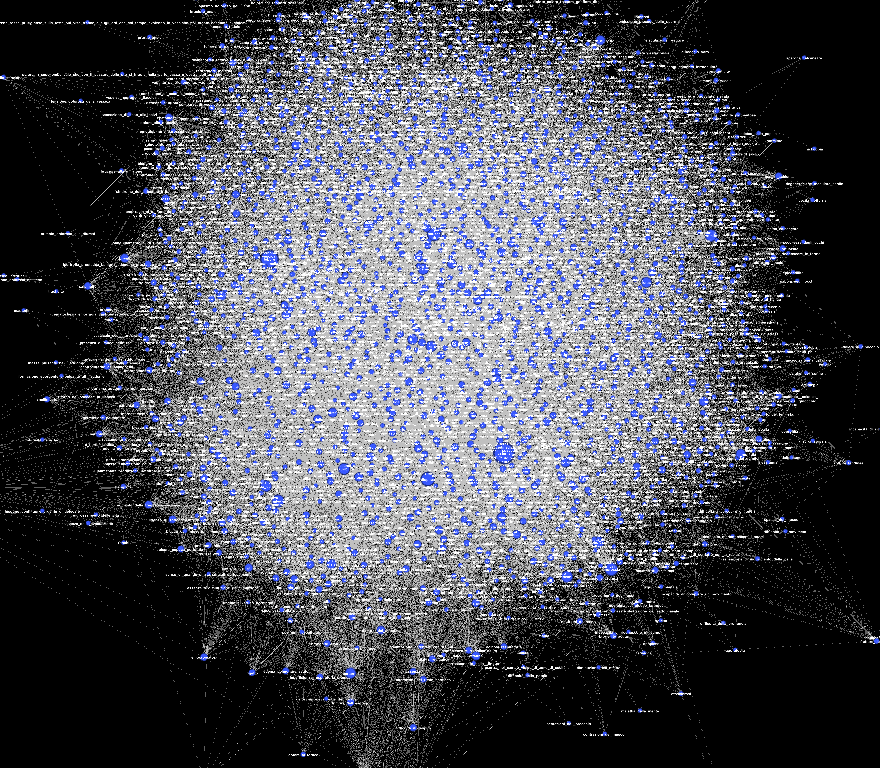
\includegraphics[width=.8\linewidth]{symnet.png}
\caption{Symptoms-disease network generated by merging of three public Italian web-pages of auto-diagnosis search engine.
The network connects symptom and disease words according to the information found in the web sites.
The network comprises \numprint{2285} nodes and more than 29k links.
Node sizes are proportional to their centrality (number of connections or degree score).
In this way the most common symptoms/diseases are represented as the biggest nodes.
}
\label{fig:net}
\end{figure}

\begin{table}[htbp]
\centering
\begin{tabular}{lccc}
\hline \rowcolor{darkgrayrow}
Disease/Symptom & degree \\
\hline
Astenia         & 384    \\
Febbre          & 313    \\
Dispnea         & 225    \\
Nausea          & 222    \\
Anoressia       & 201    \\
Ematemesi       & 193    \\
Vomito          & 182    \\
Debolezza       & 176    \\
Affaticamento   & 176    \\
Esaurimento     & 172    \\
Mancanza Forze  & 168    \\
Edema           & 158    \\
\hline
\end{tabular}
\caption{Top ranking links in \textsf{SymptomsNet}.
We can notice \quotes{periphrases/synonyms} associated to same symptoms, as \emph{Debolezza} and \emph{Mancanza Forze} which are left to increase the heterogeneity of samples in the FiloBlu project.}
\label{tab:rank}
\end{table}

In this simple example we can already notice as the most central (big) nodes are associated to the most common symptoms-diseases, as expected.
This result can be already interpreted as a validation of the performed processing.
We can notice from Tab.\ref{tab:rank} that also in the top ranking nodes we find some diseases and related synonyms: this could be an issue for the network structure, since it means that the developed processing pipeline is not able to merge together different words with equal meaning.
However, the project purpose was to create a reasonably good diseases ontology and this issue could be turned to a strength of our applications: it proves that we have an agreement between different databases (synonyms have comparable degree score and thus same importance) and it highlights the variety of mined terms (different names which identify the same disease).
In fact, this kind of occurrences allow to consider a wide range of possible synonyms in the score attribution, enforcing the text analysis required by the FiloBlu project: the node degree can be used as weight (1/degree) for text words, obtaining a simple score for the message given by the sum of the mapped keywords.

We conclude that from this very simple and preliminary work we are able to propose a novel symptoms-diseases network based on Italian public databases and, far as the author knows, no other equivalent results are reported in literature.
This work allowed also the realization of a novel database obtained by the union of publicly available data.
The extracted centrality measures can be used as weights for the corresponding symptoms/diseases and a valid input to model words frequency/importance in text analyses.

\textsf{SymptomsNet} is based on a bipartite graph which associates disease nodes to symptom ones.
These results highlight the potentiality of such structures and they leaded us to further investigate about them and their creation.
In particular, reiterating the same procedure we could be able to join together different bipartite graphs obtaining a network-of-networks structure which stores multiple types of information.
This is the main idea behind the \textsf{CHIMeRA} project.
To this purpose we have to manage more reliable data sources and improve our natural language processing pipeline to increase dataset overlaps.
All these tasks can be easier performed using English words and validated databases.
In the next sections, we are going to discuss about what natural language processing means in modern researches and we will describe the pipeline and databases used in the development of the \textsf{CHIMeRA} network-of-networks.

\end{document}
